\section{The ATLAS Detector}
\label{sec:atlas}

In this section we will extend our focus to the ATLAS detector, the general purpose
particle detector located at Point 1 of the LHC ring (see Figure~\ref{fig:p1}).
Roughly cylindrical in shape, coaxial with the beam-pipe,
the ATLAS detector is 44\,m long and 25\,m tall.
It is by far the largest such detector ever built and,
generally, is the largest and most complex device ever constructed.
Being general purpose in scope, the ATLAS detector is hermetic and has
nearly $4\pi$ radians of solid angle coverage around the $pp$ collision
point. 
Such detectors are commonly designed to have various subsystems --- \textit{subdetectors} ---
which are dedicated for the identification of specific types of particles
and interactions.
They tend to be layered about the interaction point and cylindrically symmetric
since the $pp$ interactions taking place within the detector have no preferred
direction in the plane transverse to the direction in which the proton beams
are travelling.
A view of the ATLAS detector and its subdectors is provided by Figure~\ref{fig:atlas_cutaway}.
In the following we will briefly describe each subsystem in turn, describing
first the detectors located nearer to the $pp$ collision and proceeding outwards.

\subsection{The ATLAS Coordinate System}
\label{sec:atlas_coordinate_system}

The ATLAS detector uses a right-handed coordinate system with the origin located at
the geometric center of the detector.
The $x$-axis points to the center of the LHC ring, the $y$-axis points upwards
and away from the center of the Earth, and the $z$-axis is along the beam-pipe.
The side associated with positive (negative) $z$
is referred to as the `A' (`C') side of the detector.\footnote{`A' for `airport',
since this is the side pointing towards Geneva International Airport, and
`C' for either `Crozet' or `Charly's', depending on who you ask, since this is the side
pointing towards the town of Crozet and/or Charly's Pub in the town of Saint-Genis-Pouilly.}
Due to its cylindrical symmetry, ATLAS also uses the cylindrical coordinates, $(r,\phi, z)$,
with $\phi$ the azimuthal angle about the $z$-axis and having $\phi = 0$ along the positve $x$-axis.
The spherical polar angle, $\theta$, is defined with respect to the $z$-axis, having
$\theta = 0$ parallel to the beam-pipe and $\theta = \pi/2$ in the $xy$-plane transverse
to the beam-pipe.
The pseudorapidity, $\eta$, is commonly used when describing systems of particles or locations within
the detector and is defined as $\eta = - \ln \left[ \tan \left( \theta / 2 \right) \right ]$.
The relationship between pseudorapidity and polar angle is illustrated in Figure~\ref{fig:eta_desc}.
Large (small) values of $\eta$ correspond to the \textit{forward} (\textit{central}) region of the detector.
The rapidity, $y$, is related to $\eta$ and is defined as $y = \frac{1}{2} \ln \left[ (E+p_z) / (E-p_z) \right]$.
The pseudorapidity of a particle traversing the detector is equal to its rapidity if
the particle is massless or ultra-relativistic; otherwise, they are different.
The comparison between a particle's pseudorapidity and rapidity is illustrated in
Figure~\ref{fig:eta_desc}.
The coordinates used to describe systems of particles are typically described by their
four-momenta: $(p_x, p_y, p_z)$ or, equivalently, $(\pT, \eta, \phi)$.
A distance metric commonly used to describe the distance between two systems of particles
in the detector is $\Delta R = \sqrt{ (\Delta \eta)^2 + (\Delta \phi)^2 }$. The
$\Delta R$ quantity using $y$ instead of $\eta$ is also sometimes used and will be
indicated by $\Delta R_y$.

\begin{figure}[!htb]
    \begin{center}
        \raisebox{1.5cm}{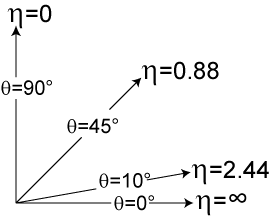
\includegraphics[width=0.35\textwidth]{figures/chapter2/eta_vs_polar}}
        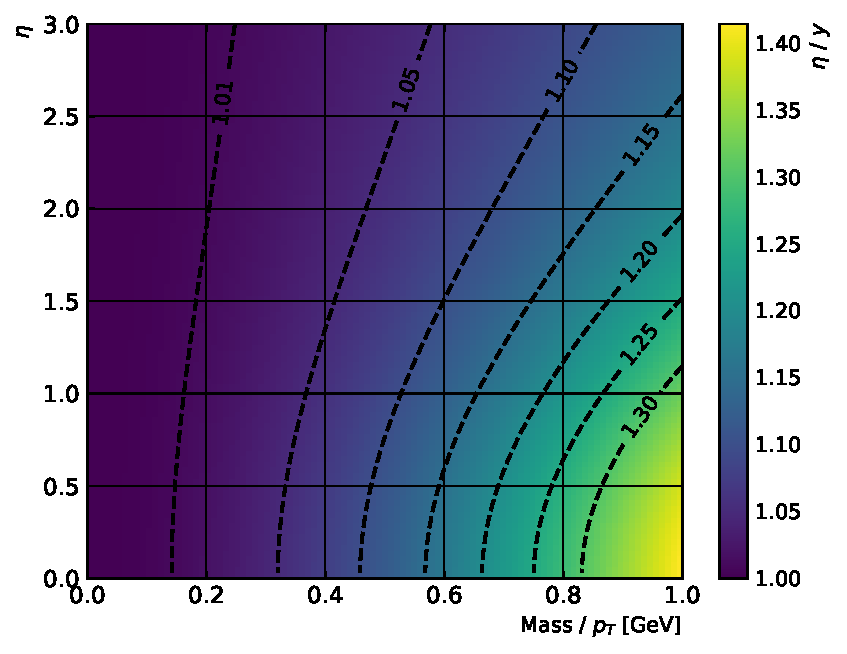
\includegraphics[width=0.55\textwidth]{figures/chapter2/eta_vs_rap}
        \caption{
            \textit{Left}: Illustration of the relationship between the pseudorapidity, $\eta$,
                and polar angle, $\theta$, defined as the angle with respect to the beam-axis ($z$-axis).
            \textit{Right}: Distribution of the ratio of a particle's pseudorapidity to its rapidity, $\eta$/$y$,
                as a function of its pseudorapidity ($y$-axis) and the ratio of its mass to its transverse momentum, \pT~($x$-axis).
        }
        \label{fig:eta_desc}
    \end{center}
\end{figure}


\begin{figure}[!htb]
    \begin{center}
        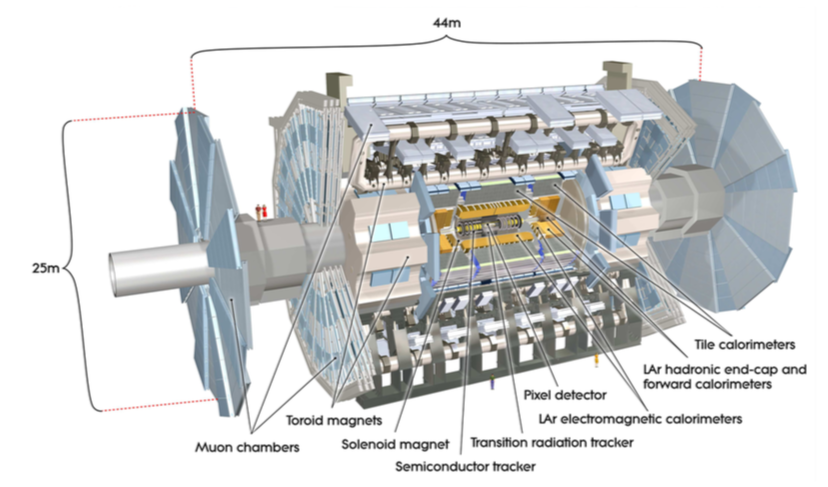
\includegraphics[width=0.95\textwidth]{figures/chapter2/atlas_cutaway}
        \caption{
            Cut-away view of the ATLAS detector with sub-systems indicated.
            Shown for comparison are figures of average-height humans standing
            at the feet of the detector and standing on the forward shielding
            between the big wheels of the forward muon system.
        }
        \label{fig:atlas_cutaway}
    \end{center}
\end{figure}


\begin{figure}[!htb]
    \begin{center}
        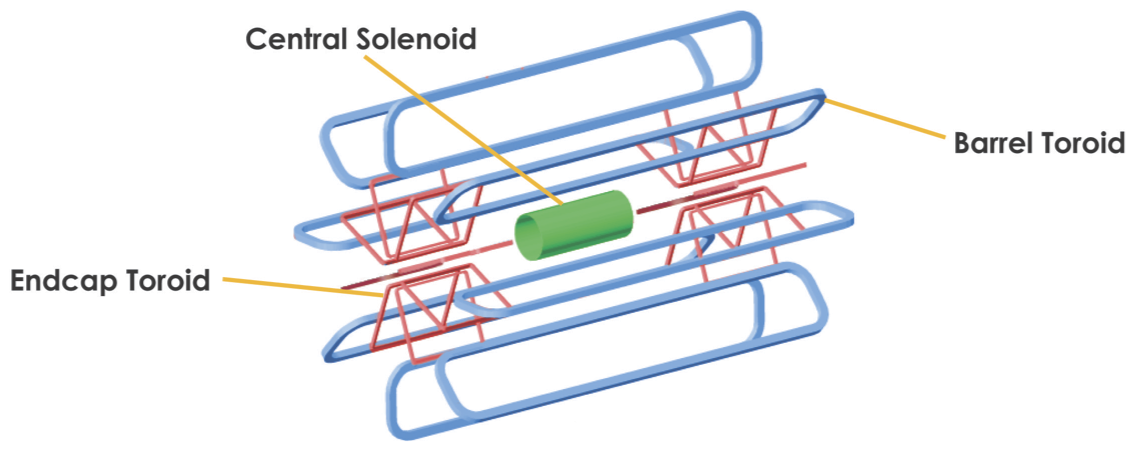
\includegraphics[width=0.95\textwidth]{figures/chapter2/atlas_magnet_system}
        \caption{
            A view of the ATLAS magnet system. Shown are the 2\,T solenoid magnet
            in green, the barrel toroid system in blue, and endcap toroid magnets
            in red.
        }
        \label{fig:atlas_magnet_system}
    \end{center}
\end{figure}

%%%%%%%%%%%%%%%%%%%%%%%%%%%%%%%%%%%%%%%%%%%%%%%%%%%%%%%%%%%%%%%%%%%%%
%%%%%%%%%%%%%%%%%%%%%%%%%%%%%%%%%%%%%%%%%%%%%%%%%%%%%%%%%%%%%%%%%%%%%
%
% INNER DETECTOR
%
%%%%%%%%%%%%%%%%%%%%%%%%%%%%%%%%%%%%%%%%%%%%%%%%%%%%%%%%%%%%%%%%%%%%%
%%%%%%%%%%%%%%%%%%%%%%%%%%%%%%%%%%%%%%%%%%%%%%%%%%%%%%%%%%%%%%%%%%%%%
\subsection{The Inner Detector}
\label{sec:inner_detector}

The innermost subdetector of ATLAS is the Inner Detector (ID)~\cite{Haywood:331064}.
The ID covers the region $\lvert \eta \rvert < 2.5$ and is composed, in order
of increasing radial distance from the beam-pipe, of the pixel detector,
semiconductor tracker (SCT), and the transition radiation tracker (TRT).
These detectors enable the reconstruction of the tracks associated with
the $\mathcal{O}(1000)$ charged particles emerging from each $pp$ bunch collision, occuring
every 25\,ns.
An illustration of the ID and its subdetectors is shown in Figure~\ref{fig:atlas_inner_detector}.
Additional, more detailed views of the barrel and endcap sections of the ID are shown in Figure~\ref{fig:atlas_ID_exploded}.
The ID is situated inside of the central solenoid, indicated in Figure~\ref{fig:atlas_magnet_system},
which provides an axial 2\,T magnetic field and extends over a length of 5.3\,m with a diameter of 2.5\,m.
The bending of charged particles in the $xy$-plane due to the presence of the solenoidal
field allows for their momenta to be measured using the curvature of their reconstructed tracks.

\begin{figure}[!htb]
    \begin{center}
        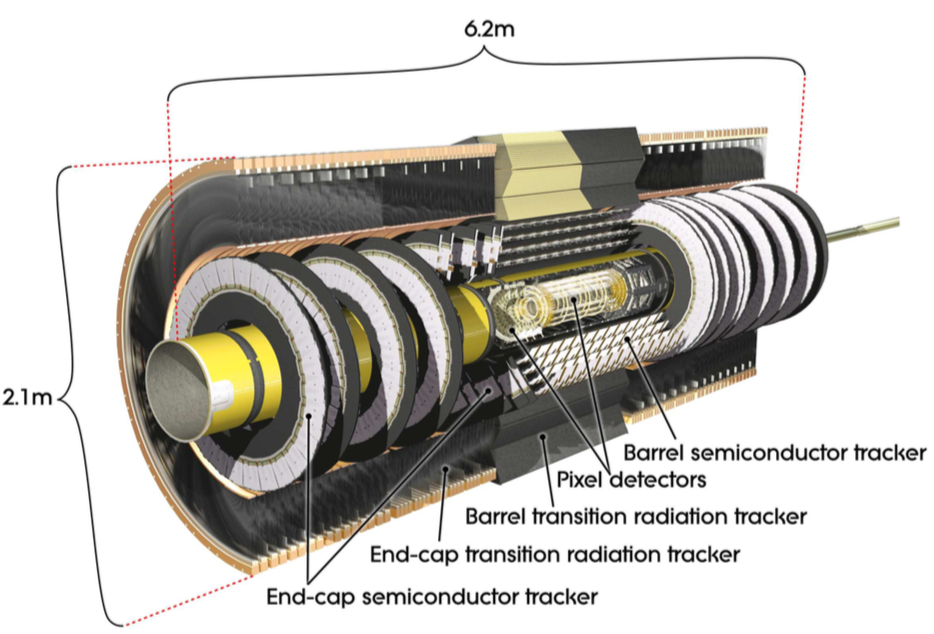
\includegraphics[width=0.75\textwidth]{figures/chapter2/atlas_inner_detector}
        \caption{
            Cross-sectional view of the ATLAS inner detector. Shown are the barrel
            and end-cap portions of the pixel, SCT, and TRT detectors.
        }
        \label{fig:atlas_inner_detector}
    \end{center}
\end{figure}

\begin{figure}[!htb]
    \begin{center}
        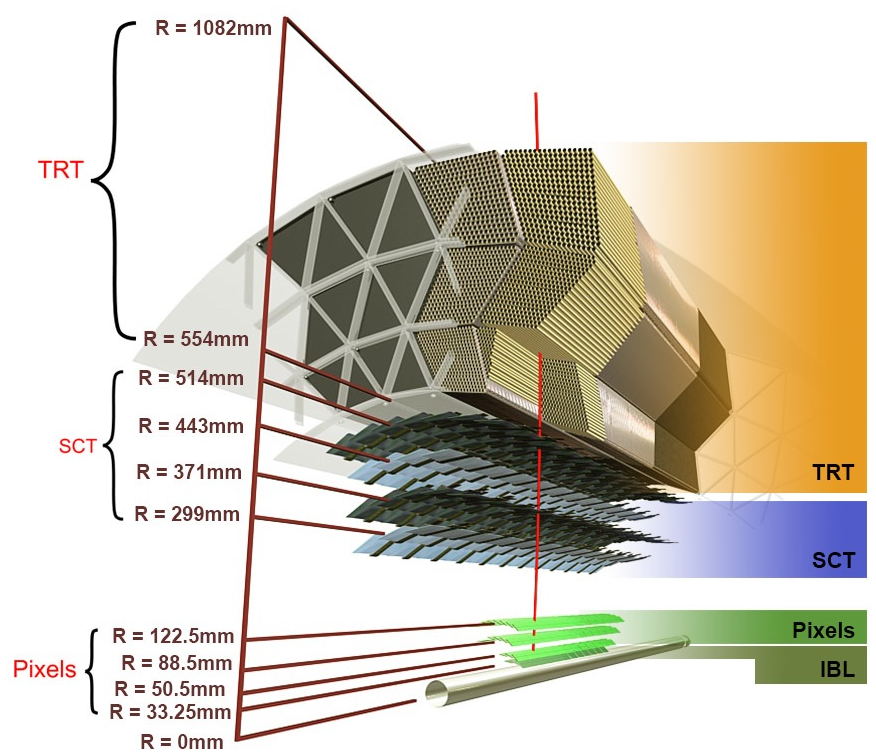
\includegraphics[width=0.6\textwidth]{figures/chapter2/atlas_ID_barrel_exploded}
        \raisebox{1.4cm}{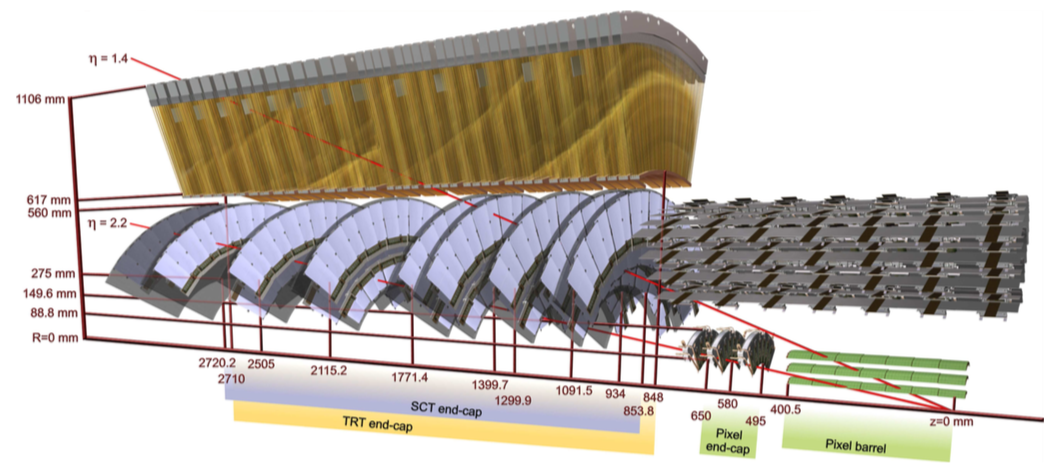
\includegraphics[width=0.85\textwidth]{figures/chapter2/endcap_ID_exploded}}
        \caption{
            Exploded views of the barrel (\textit{left}) and endcap (\textit{right}) portions
            of the inner-detector.
        }
        \label{fig:atlas_ID_exploded}
    \end{center}
\end{figure}

\subsubsection{The Pixel Detector and IBL}
\label{sec:id_pixel}

The pixel detector is the innermost subdetector of the ID, situated very near to and surrounding
the beam-pipe.
It is composed of three separate sections: a barrel section and two end-cap sections.
The barrel section  of the pixel detector has a cylindrical geometry and the end-cap sections
are disks centered on the beam-pipe.
The barrel section has four layers, each with increasing radius, and there are three disks in each
of the end-caps. This ID geometry, shown in Figure~\ref{fig:atlas_ID_exploded}, covers
the region $\lvert \eta \rvert < 2.5$.

The pixel detector, being so near the $pp$ collisions, is subject to the highest particle
fluxes of any other subsystem.
As a result, it is built to have very fine granularity: its sensing elements consist of
$250$\,\micron~thick detectors housing pixels of reverse-biased n-type semiconductor material,
each having a nominal size of $50\times400\,\micron^2$.
In total, there are roughly 80 million channels read out from the pixel detector alone.
This allows for the pixel detector's fine spatial hit resolution of $10\,\micron$ in
$(r-\phi)$ and $115\,\micron$ along $z$.

The innermost layer of the pixel detector's barrel section is referred to as the
\textit{Insertable B-Layer} (IBL), and was installed at the beginning of the Run-II
data-taking period~\cite{Capeans:1291633}.
It corresponds, essentially, to the instrumentation of the ATLAS beam-pipe, as seen in Figure~\ref{fig:pixel_detector_trans},
and is located at a radial distance of 3.3\,cm.
It alone accounts for 8 million readout channels of
the pixel detector --- resulting in an ultra precise spatial hit resolution of $8\,\micron$ in $(r-\phi)$ and
$40\,\micron$ along $z$.
Beyond improving the overall measurements and reconstruction of charged particle tracks,
the IBL was installed in order to improve the performance of secondary vertex
reconstruction --- an essential ingredient to the algorithms associated with
the reconstruction and identification of jets originating from the decays
of $b$-hadrons whose decays occur at radial distances frequently beyond that
of the IBL.



\begin{figure}[!htb]
    \begin{center}
        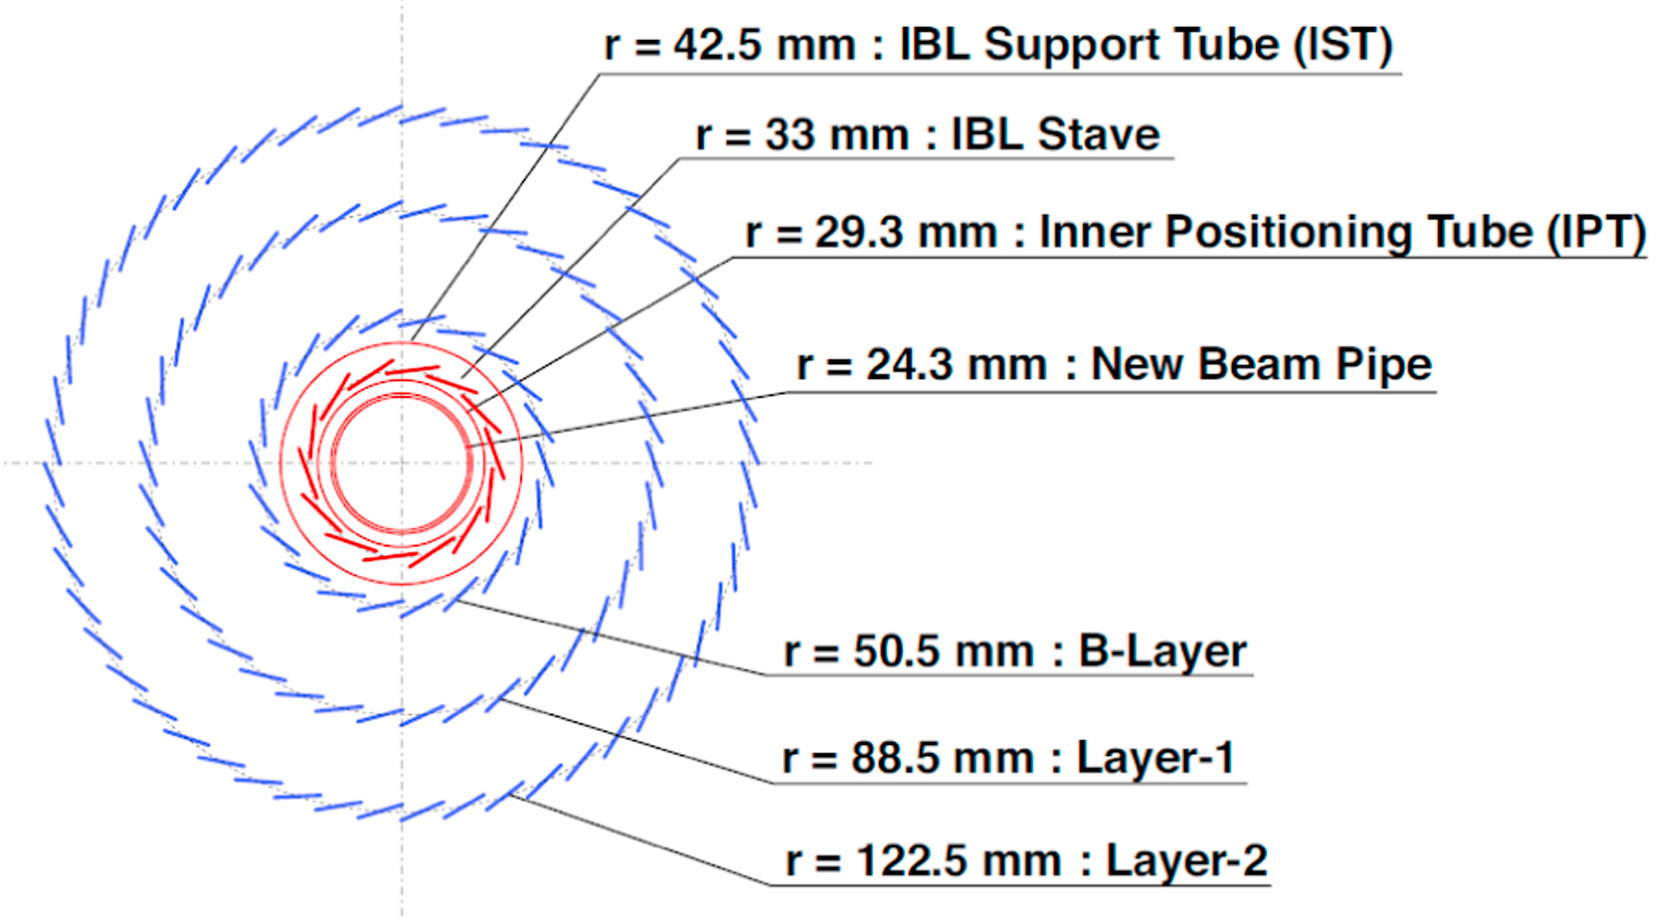
\includegraphics[width=0.8\textwidth]{figures/chapter2/pixel_detector_trans}
        \caption{
            Transverse view of the barrel section of the pixel detector, showing
            the innermost layer, the Insertable B-Layer (IBL) (red), and the
            three surrounding layers (blue). From Ref.~\cite{Backhaus:2016ctq}.
        }
        \label{fig:pixel_detector_trans}
    \end{center}
\end{figure}


